\begin{savequote}[75mm]
Orice aplicație ce \emph{poate} fi scrisă în JavaScript, \emph{va fi},
la un moment dat, scrisă în JavaScript.
\qauthor{Jeff Atwood}
\end{savequote}

\chapter{JavaScript și AngularJS}

JavaScript, un limbaj de programare controversat, a ajuns să fie 
cel mai important limbaj al web-ului. AngularJS este un framework
JavaScript creat de Google pentru a depăși limitările HTML-ului și pentru a
ușura crearea aplicațiilor SPA. În acest capitol voi descrie aceste
două tehnologii.


\section{JavaScript}

JavaScript, cunoscut și ca ECMAScript, a fost creat în 1995, 
de Brendan Eich, pentru Netscape. În ciuda
numelui, JavaScript nu are nimic în comun cu Java în afară de sintaxa
inspirată de C.

Brendan Eich, un iubitor al limbajelor funcționale, își dorea să creeze
un limbaj asemănător cu \emph{Scheme}\footnote{\url{http://en.wikipedia.org/wiki/Scheme\_(programming\_language)}}, care este un dialect a lui 
\emph{Lisp}\footnote{\url{http://en.wikipedia.org/wiki/Lisp\_(programming_language)}}. 
Netscape avea însă alte scopuri. JavaScript a apărut în perioada în care
se credea că applet-urile Java vor cuceri lumea, iar Netscape dorea un limbaj
interpretat, dinamic, ca o alternativă mai puțin intimidantă a lui Java,
pentru programatorii amatori.

Astfel, Eich a fost nevoit să creeze un limbaj cu o sintaxă bazată pe cea
a lui C, dar iubirea lui a față de limbajele funcționale poate fi observată
totuși în JS. JS este unul din primele limbaje folosite la scară mare
care are funcții anonime (cunoscute și ca expresii lambda). Java a introdus
funcțiile anonime abia în 2014, în versiunea 8.

Faptul că JS a încercat să fie un limbaj de programare adresat
și amatorilor, a avut niște consecințe negative pentru limbaj.
Limbajul încearcă să fie iertător atunci cu un programator ce
nu știe ce face, lucru care care a dus la comportamentul neașteptat
al limbajului pentru un programator care știe ce face.
Mult timp, comunitatea programatorilor
i-a privit pe programatorii JavaScript ca fiind amatori.

Pe lângă toate astea, JS a fost mereu asociat cu API-ul de manipulare al DOM-ul 
(Document Object Model)\footnote{\url{http://en.wikipedia.org/wiki/Document\_Object\_Model}},
care a fost implementat în mod diferit
de fiecare browser, lucru care a făcut ca programarea în JS să fie
grea și neelegantă.

Din aceste motive, nu mulți s-ar fi așteptat ca, dintre toate
limbajele, JS să devină cel mai popular și mai căutat limbaj din
lume. Dar s-a întâmplat. Mai întâi, Ajax l-a adus în prim-plan.
jQuery\footnote{\url{https://jquery.com/}}, o librărie scrisă în JavaScript, a venit să simplifice 
Ajax și să ascundă diferențele dintre
browsere. Partea de front-end a aplicațiilor a devenit din ce
în ce mai complexă, astfel tot mai mulți programatori au
devenit interesați de ea, ducând la librării din ce în ce mai bune.

Pe partea de client, JS este câștigător incontestabil, fiind
singurul limbaj cunoscut de toate browser-ele în mod nativ.
Singura alternativă o reprezintă limbajele care sunt compilate
în JS, cum ar fi CoffeeScript, ClojureScript etc, dar acestea
sunt mult mai puțin folosite. Pentru ele, JS este
noul limbaj de asamblare.

Pe lângă faptul că JS este de departe cel mai folosit limbaj
pe browser, acesta nu s-a oprit aici. JavaScript a "scăpat" din browser.
Prin intermediul lui Node.js\footnote{\url{https://nodejs.org}}, 
o tehnologie ce capătă amploare 
din ce în ce mai mare, JavaScript poate fi folosit
și pe server. 

MEAN\footnote{\url{http://mean.io}} (MongoDB Express Angular.js Node.js) 
este o combinație de tehnologii
care îi face pe dezvoltatori să se bucure de avantajele folosirii
unui singur limbaj la toate nivelele aplicației, de la front-end,
trecând prin back-end și până în baza de date. Acesta a fost numit
de unii ca fiind noul 
LAMP\footnote{\url{http://en.wikipedia.org/wiki/LAMP\_(software\_bundle)}}
(Linux Apache MySQL PHP).

\begin{figure}[t]
  \centering
    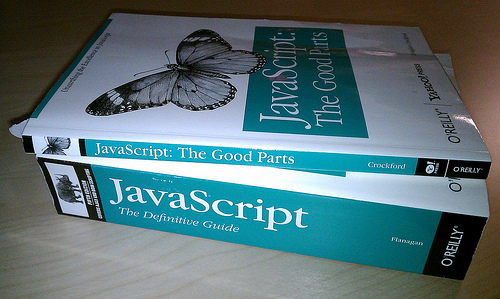
\includegraphics[width=1\textwidth]{./chap3-code/js}
  \caption{Părțile bune din JavaScript}
\end{figure}

În concluzie, indiferent de părerile personale și dacă ne place
sau nu, un lucru este cert: în momentul de față, JavaScript
este cel mai important jucător din lumea limbajelor
de programare. JavaScript este pe locul 1 la numărul de
repositories pe GitHub și cel mai căutat limbaj de programare
în anunțurile de angajare.

\section{AngularJS}

În această secțiune voi trece foarte rapid peste componentele
de bază ale lui AngularJS. Scopul secțiunii 
este sublinierea elementelor
esențiale ale lui Angular: șabloane, directive, controllere,
servicii.


AngularJS este un framework MVC ce folosește HTML-ul ca bază pentru
limbajul său de șabloane. El extinde HTML-ul cu structuri de control,
de exemplu pentru iterare și permite și definirea de noi \emph{directive},
care pot fi elemente sau atribute HTML.

În continuare prezint o mică porțiune din codul tutorialului oficial Angular, disponibil la 
\url{https://docs.angularjs.org/tutorial/step_11}.

\lstinputlisting[language=HTML, title=app/index.html, numbers=left]{chap3-code/index.html}
\lstinputlisting[title=app/js/services.js, numbers=left]{chap3-code/services.js}
\lstinputlisting[title=app/js/controllers.js, numbers=left]{chap3-code/controllers.js}

În \texttt{index.html}, linia 1, prin intermediul atributului HTML \texttt{ng-controller}
(ce corespunde directivei Angular \texttt{ngController}) Angular
află că pentru toate elementele din interiorul elementului
body, scope-ul este luat din controller-ul cu numele
\texttt{PhoneListCtrl}, definit în fișierul 
\texttt{app/js/controllers.js} (linia 4).

Linia 4 din \texttt{index.html} folosește directiva \texttt{ngRepeat} pentru
a itera prin array-ul cu numele \texttt{phones} de pe \texttt{scope}-ul curent.
Acest array este declarat în \texttt{controllers.js}, linia 6.

În \texttt{controllers.js}, linia 5, \texttt{'Phone'} este pasat
ca argument al funcției în interiorul unui array. Acest lucru
îi spune framework-ului să injecteze serviciul \texttt{Phone},
definit în \texttt{app/js/services.js}, linia 5.
Acest serviciu se folosește de \texttt{ngResource} pentru a
crea mai multe metode ce apelează un API REST aflat la adresa
\texttt{/phones}. Astfel, deși uitându-ne în controller putem
avea senzația că \texttt{\$scope.phones} este populat sincron,
în realitate, metoda \texttt{query} din serviciu face un HTTP GET
la adresa \texttt{/phones} de unde un obiect JSON este returnat,
iar \texttt{\$scope.phones} este populat cu acest obiect.

